\documentclass{ws-ijcm}
%\documentclass{article}

%\usepackage{hyperref}

\usepackage{multirow}

\usepackage{graphicx}

\usepackage{amsmath}

\usepackage[round,authoryear]{natbib}
\bibliographystyle{unsrtnat}

%\usepackage{authordate1-4}

%\usepackage{amssymb}
%\usepackage{amsthm}

\newcommand{\bfr}{\mathbf{r}}
\newcommand{\bfu}{\mathbf{u}}

\newcommand*{\Ab}{\overline{A}}
\newcommand*{\Abb}{\overline{\overline{A}}}

%\def\volumeyear{2017}

%\def\baselinestretch{2} 


\begin{document}

%%%%%%%%%%%%%%%%%%%%% Publisher's Area please ignore %%%%%%%%%%%%%%%
%
\catchline{}{}{}{}{}
%
%%%%%%%%%%%%%%%%%%%%%%%%%%%%%%%%%%%%%%%%%%%%%%%%%%%%%%%%%%%%%%%%%%%%

\markboth{D.~Duque, P.~Espa\~nol}{Assignment that preserves field values}

\title{AN ASSIGNMENT PROCEDURE FROM PARTICLES TO MESH THAT PRESERVES
  FIELD VALUES}


\author{DANIEL DUQUE\footnote{
  ETSI Navales, Universidad Polit\'ecnica de Madrid,
  Avd.  de la Memoria 4, Ciudad Universitaria  - 28040  Madrid, Spain. \email{daniel.duque@upm.es}}}

\address{%
  Model Basin Research Group (CEHINAV).
  ETSI Navales, Universidad Polit\'ecnica de Madrid.
  Madrid, Spain
}
%\email{daniel.duque@upm.es}

\author{PEP ESPA\~NOL}

\address{%
  Dpto. de F{\'\i}sica Fundamental.
  Universidad Nacional de Educaci\'on a Distancia.
  Madrid, Spain}



\maketitle

\begin{history}
\received{(Day Month Year)}
\revised{(Day Month Year)}
\end{history}


\begin{abstract}
  In Computational Fluid Dynamics there have been many attempts to
  combine the advantages of having a fixed mesh, on which to carry out
  spatial calculations, with using particles moving according to the
  velocity field. These ideas in fact go back to Particle-in-Cell
  methods, proposed about 60 years ago.
%  
  Of course, some procedure is needed to transfer field information
  between particles and mesh. There are many possible choices for this
  ``assignment'', or ``projection''.
%
  Several requirements may guide this choice. Two well-known ones are
  conservativity and stability, which apply to volume integrals of the
  fields.
%
  An additional one is here considered: preservation of
  information. This means that assignment from the particles onto
  the mesh and back should yield the same field values when the particles
  and the mesh coincide in position.
%  
  The resulting method is termed ``mass'' assignment, due
  to its strong similarities with the Finite Element Method.
%
  Several procedures are tested, including the well-known FLIP, on
  three scenarios: simple 1D convection, 2D convection of Zalesak's
  disk, and a CFD simulation of the Taylor-Green periodic vortex
  sheet.  Mass assignment is seen to be clearly superior to other
  methods.
%
\end{abstract}


\keywords{%
Finite element	; %
Particle method	; %
Eulerian	; %
Lagrangian	; %
Navier-Stokes	; %
Incompressible flow}

%\begin{keyword}
%a \s b \sep c
%
%\PACS 71.33 \sep 71.46
%\end{keyword}



\section{Introduction}
\label{sec:intro}

Historically, there have been two points of view to describe the
dynamics of fluids. In the Eulerian picture, the dynamics of a fluid
is described with respect to an external frame. In the Lagrangian
picture the dynamics is described with respect to the flow. These two
approaches are reflected in computational fluid dynamics (CFD), in
which the spatial discretization may be carried out on a fixed,
Eulerian, mesh, or on a Lagrangian set of moving particles. Each
approach has its advantages and drawbacks (\cite{violeau2012fluid}.)

It is therefore natural to try to combine the best of both approaches.
For example, the numerically expensive calculations related to spatial
derivatives could be carried on a fixed mesh. The velocity field would
then be transferred to particles, which would move according to it,
advecting other fields. These would be transferred back to the mesh to
begin the next iteration. This idea goes back to Particle-in-Cell
(PIC) methods, introduced in the 1950s, see Refs.
\cite{evans1957,PIC2}.

However appealing, this idea also has its drawbacks. The obvious one
is that an additional procedure is needed to transfer the field
information between particles and mesh. This procedure has been termed
``assignment'' --- the term ``projection'' will be used as a synonym,
as is customary in this field. However, the latter could lead to
confusion with other procedures, such as the Galerkin projection
(see e.g. \cite{rapun2010reduced}), in which a continous set of equations
is projected on a functional space (even if, as we show below, some
similarities may exist between the Galerkin procedure and our ``mass''
assigment.)

Our main task is to study the performance of different projection
techniques, under the guidance of several requirements. One of them is
conservativity: the total volume integral of a field must not vary
upon projection. Another is stability: the integral of the square of
any field should decrease upon projection. These two requirements are
well known, while here an additional one is considered: preservation
of information. This means that the field values at discrete points do
not vary under reconstruction (extension to the continuum) followed by
projection. This is enforced both for reconstruction from the mesh
followed by projection back onto the mesh, and for the equivalent
procedure from the particles. Another view of this property is that,
if the particles' positions coincide with the mesh nodes, then for
assignment from the particles onto the mesh, and back, will leave
the field values invariant.

The article is organized as follows. In Section \ref{sec:assignment}
different assignment procedures are discussed, together with the
requirements.
%
These procedures are then tested in three scenarios in Section
\ref{sec:results}: a very simple 1D convection of a step function,
Zalesak's disk 2D test, and a CFD simulation of the Taylor-Green
periodic vortex sheet, a solution of the Navier-Stokes equations
%
Some finishing remarks are given in Section \ref{sec:conclusions}.



\section{Assignment procedures}
\label{sec:assignment}

In Subsection \ref{sec:functions} a general framework for assignment
through functional sets is provided. The requirements of
conservativity and stability will be discussed in Subsection
\ref{sec:cons_stab}. The simplest assignment is introduced in
\ref{sec:delta_assignment}. The FLIP procedure
(Refs. \cite{brackbill1986flip,brackbill1988}), which is currently very
popular in the computer graphics community (see
e.g. \cite{bridson_2015}) is considered in Subsection
\ref{sec:flip_assignment}.  In Subsection \ref{sec:mass_assignment}
the additional requirement of preservation of information is
introduced, thus leading to mass assignment.
%and its possible variants.


\subsection{Assignment functions}
\label{sec:functions}

%We will use the following convention for nodal functions.

A set of functions $\{\psi_\mu\}$ will be used to \emph{reconstruct} a
field $A(\bfr)$ from its values at particles $A_\mu$:
\begin{equation}
\label{eq:part_interp}
A(\bfr) \doteq \sum_\mu A_\mu \psi_\mu ( \bfr ) .
\end{equation}

The functions are supposed to comply with partition of unity, in order
a particle distribution with constant values yields a constant field:
\begin{equation}
\label{eq:sum_psi}
\sum_\mu \psi_\mu(\bfr) = 1 .
\end{equation}
In this work, only the simple linear Finite Element basis functions
(FEs) will be considered , even though other choices are of course
possible. These are piece-wise affine functions, which in 1D are equal
to $1$ at each particles, then linearly decrease to $0$ at the two
neighboring nodes.  In 2D they are pyramids of height $1$ at each
particle, decreasing to $0$ at the neighboring nodes. The Delaunay
triangulation is used in order to precisely define neighbors.

For the mesh the same symbols will be kept, but the sub-indices will
be Latin letters. A field is reconstructed from the values at mesh
nodes $\Ab_i$ by mesh functions $\{\psi_i\}$:
\begin{equation}
\label{eq:mesh_interp}
\Ab(\bfr) \doteq \sum_i \Ab_i \psi_i ( \bfr ) .
\end{equation}

The particle-to-mesh assignment procedure consists in finding nodal
values for $\Ab_i$ given particle values $A_\mu$. The inverse
mesh-to-particle yields particle $\Abb_\mu$ given mesh $\Ab_i$.

%In addition, both particles and mesh nodes may be endowed with
%volumes, and perhaps other functions, their definition depending on
%the method.



\subsection{Conservativity and stability}
\label{sec:cons_stab}

An property that may lead us on our research of possible assignment
methods is conservativity, in the sense of \cite{cottet2000}: that the
integral of a field does not change on projection. Integrating field
$A$ of Eq. (\ref{eq:part_interp}),
\[
\int A(\bfr) d\bfr  =  \sum_\mu A_\mu v_\mu ,
\]
where particle volumes are given by
\begin{equation}
  \label{eq:part_v}
  v_\mu := \int \psi_\mu(\bfr) d\bfr .
\end{equation}
%
Equivalently, mesh volumes may be defined from
Eq. (\ref{eq:mesh_interp}),
\begin{equation}
  \label{eq:mesh_v}
  v_i := \int \psi_i(\bfr) d\bfr .
\end{equation}
(As shown below, the FLIP method does \emph{not} use this definition
of the mesh volume.)


Whichever the particular definition of the volumes, conservativity is
expressed as:
\begin{equation}
\label{eq:cons}
\sum_i \Ab_i v_i = \sum_\mu A_\mu v_\mu .
\end{equation}

When applied to the components of the linear momentum, this would
guarantee the global conservation of linear momentum. For a density
field, this would guarantee conservation of mass. It therefore would
seem as a vital requirement. However, it will be seen that methods
that do not comply with this condition still may deviate little from
it in practice.

Of course, the same requirement could be asked when projecting from the
mesh onto the particles:
\begin{equation}
\label{eq:cons2}
\sum_\mu \Abb_\mu v_\mu  = \sum_i \Ab_i v_i .
\end{equation}

Another requirement is stability: for any energy-like expression
defined on the particles and on the mesh:
\[
E_\mathrm{p} := \sum_\mu v_\mu A_\mu^2 \qquad
E_\mathrm{m} := \sum_i v_i \Ab_i^2 ,
\]
we require
\begin{equation}
\label{eq:stab}
E_\mathrm{m} \le E_\mathrm{p} .
\end{equation}
This guarantees that there is no overshoot in e.g. the kinetic energy
upon assignment, i.e. that the assigment process is disipative.  For a
general field this enforces a diminishing second momentum, which
prevents overshooting in a global sense. Of course, the same could be
required when going from the mesh to the particles.

\subsection{$\delta$ assignment}
\label{sec:delta_assignment}

The simplest assignment would be to define mesh values as the local
values reconstructed from the particles:
\begin{equation}
\label{eq:delta}
\Ab_i = \Ab(\bfr_i) = \sum_\mu A_\mu \psi_\mu( \bfr_i ) .
\end{equation}
Also,
\begin{equation}
\label{eq:delta2}
\Abb_\mu = \Abb(\bfr_\mu) = \sum_i \Ab_i \psi_i( \bfr_\mu ) .
\end{equation}

Particle volume may simply be defined as in (\ref{eq:part_v}) and
(\ref{eq:mesh_v}). It is easy to check that this procedure does not
satisfy either conservativity or stability.  It is, nevertheless, very
simple to implement, and was the method used in our previous study,
\cite{duque_2017b}. In Table \ref{table:methods} the relevant
expressions for this method is shown, along others for methods that
will be considered next.

\begin{table}
  \centering
  \begin{tabular}{|c|c|c|}
    \hline
     method    &  part $\rightarrow$ mesh  & mesh $\rightarrow$ part    \\
     \hline
     \hline
     $\delta$  &
     $\displaystyle \Ab_i = \sum_\mu A_\mu \psi_\mu ( \bfr_i )$   (\ref{eq:delta} )  &
     \\
     FLIP &
     $\displaystyle \Ab_i :=  \sum_\mu A_\mu v_\mu \psi_i(\bfr_\mu) /\sum_\mu v_\mu \psi_i(\bfr_\mu)$ (\ref{eq:PIC},\ref{eq:FLIP_vol})
     &
     \multirow{3}{*}{$\displaystyle \Abb_\mu = \Abb(\bfr_i) = \sum_i \Ab_i \psi_i ( \bfr_\mu )$ (\ref{eq:delta2})}
     \\
     mass-$\delta$ &
     $\displaystyle \Ab_i := \sum_j m_{ij}^{-1} \int d\bfr A(\bfr) \phi_j(\bfr)$
     (\ref{eq:proj}, \ref{eq:phi_def}) &
     \\
     \hline
     full mass &
     $\displaystyle \Ab_i := \sum_j m_{ij}^{-1} \int d\bfr A(\bfr) \psi_j(\bfr)$
     (\ref{eq:proj}, \ref{eq:phi_def}) &
     $\displaystyle \Abb_\mu := \sum_\nu m_{\mu\nu}^{-1} \int d\bfr \Ab(\bfr) \psi_\nu(\bfr)$
     (\ref{eq:proj2}) \\
     \hline
     \hline
     mass - lumped &
     $\displaystyle \Ab_i := \sum_j m_{ij}^{-1} \int d\bfr A(\bfr) \psi_j(\bfr)$
     (\ref{eq:proj}, \ref{eq:phi_def}) &
     \multirow{2}{*}{$\displaystyle \Abb_\mu := \frac1{v_\mu} \int d\bfr \Ab(\bfr) \psi_\mu(\bfr)$}
     (\ref{eq:lumped}) \\
     lumped &
     $\displaystyle \Ab_i := \frac1{v_i} \int d\bfr A(\bfr) \psi_i(\bfr)$
     (\ref{eq:proj}, \ref{eq:lumped}) &
     \\
     \hline
  \end{tabular}
  \caption{Features of the methods considered (left column), the procedure
    by which fields are projected from particles to mesh (middle column), and the reverse
    procedure (right column). References are given to relevant equations in the text.
    The last two methods have been tested, but results are not given here, for b revity.
    \label{table:methods}}
\end{table}




\subsection{FLIP assignment}
\label{sec:flip_assignment}

This procedure starts from the expression
\begin{equation}
\label{eq:PIC}
\Ab_i :=  \frac{1}{v_i} \sum_\mu A_\mu v_\mu \psi_i(\bfr_\mu) .
\end{equation}
The particle volumes may be defined as in (\ref{eq:part_v}).  If
(\ref{eq:mesh_v}) is used for the mesh volumes, the PIC expression is
recovered (see Refs. \cite{evans1957,PIC2}).

The FLIP procedure proposes the alternative mesh volume:
\begin{equation}
\label{eq:FLIP_vol}
v_i := \sum_\mu v_\mu \psi_i(\bfr_\mu) .
\end{equation}

This procedure can be shown to satisfy both conservativity and
stability.

A later projection onto the particles is exactly as in the
$\delta$-assignment, Eq. (\ref{eq:delta2}), and this can be seen to
again satisfy conservativity and stability.

This procedure may seem to be a great improvement since a simple
change in the mesh volume restores conservativity and stability.  It
is also convenient to code, since the same mesh functional set,
$\{\psi_i\}$, is used for both particle to mesh assignment and its
reverse.  However, it may seem somewhat strange that the volume
of a nodal mesh (\ref{eq:FLIP_vol}) does
not depend on the mesh itself, but on the particles around it.  A node
may even have a vanishing volume if no particles are close to it and the
$\{\psi_\mu\}$ have compact support.  Also, the two assignments,
(\ref{eq:delta2}) and (\ref{eq:PIC}) are clearly unsymmetrical.
A summary of the method is given in Table \ref{table:methods}.



\subsection{Mass assignment}
\label{sec:mass_assignment}

Let us consider the assignment procedure
\begin{equation}
\label{eq:proj}
\Ab_i :=  \int d\bfr A(\bfr) \phi_i(\bfr) .
\end{equation}

Here, the assignment functional set $\{ \phi_i(\bfr) \}$ consists of
normalized functions:
\begin{equation}
\label{eq:delta_norm}
\int d\bfr \phi_i(\bfr) = 1 ,
\end{equation}
so that a constant field yields constant mesh values.  Notice the
$\{\psi_\mu\}$ functions carry no physical units, but the
$\{\phi_\mu\}$ have units of length$^{-d}$, where $d$ is the spatial
dimension.  The $\delta$ method is recovered as a special case if
Dirac $\delta$ functions are used,
$ \phi_i(\bfr) = \delta(\bfr-\bfr_i)$, which in retrospect explains
its name.

For conservativity, let us evaluate
\begin{equation}
\label{eq:cons_check}
\sum_i \Ab_i v_i =
\sum_i
\left(
  \int d\bfr A(\bfr) 
\right)
\phi_i(\bfr) v_i =
\int d\bfr A(\bfr)
\left(
 \sum_i \phi_i(\bfr) v_i 
\right) .
\end{equation}
If the last parenthesis was equal to $1$, conservativity would apply
(with particle volumes as in (\ref{eq:part_v}). Therefore, these
functions must satisfy
\begin{equation}
\label{eq:delta_sum}
\sum_i v_i \phi_i(\bfr) = 1 .
\end{equation}
If this condition holds, it is straightforward to proof that stability
is also satisfied.

The simplest way to define these functions would be as normalized
versions of the $\{ \psi_i \}$ :
\begin{equation}
\label{eq:lumped}
  \phi_i(\bfr) = \frac1{v_i}  \psi_i(\bfr) 
\end{equation}
%This, however, yields methods that do not satisfy s
This would correspond to a ``lumped mass'' method, a term that will
become clear very soon.

Let us however consider $\{\phi_i\}$ that ``preserves nodal
information''. This means that that a reconstruction procedure,
followed by projection, should leave the nodal values invariant:
\begin{equation*}
%\label{eq:lumped}
\Ab_i :=  \int d\bfr  \phi_i(\bfr) \left(\sum_j \Ab_j \psi_j(\bfr) \right) .
\end{equation*}
(See also \cite{cottet2000} , p. 243, for an application of this
idea to an iterative method.)  Notice these two operations are carried
out on the mesh only (or, on particles only). It is, in general,
impossible to satisfy this requirement for a projection from the mesh
onto the particles, back onto the mesh (or its equivalent, starting
from the particles.) Alternatively, the two operations may be thought
of as taking place for the spacial situation in which the particles'
position coincide with the mesh nodes. This is indeed a common choice
for the initial configuration of a simulation, and also for methods in
which particles are re-created at each time step.

This means
\begin{equation}
\label{eq:ortho}
\int d\bfr \phi_i(\bfr) \psi_j(\bfr) = \delta_{ij} ,
\end{equation}
where the latter $\delta$ is Kronecker's. This will be called the
``preservation property''.  If the $\{\phi_i\}$ are linear
combinations of the $\{\psi_i\}$ set, it is simple to show that
\begin{equation}
\label{eq:phi_def}
\phi_i(\bfr) = \sum_j m_{ij}^{-1} \psi_j(\bfr) ,
\end{equation}
where the inverse of the mass matrix appears, the latter defined as
having elements
\[
m_{ij} =:  \int d\bfr  \psi_i(\bfr)   \psi_j(\bfr) .
\]

It can be shown that the functions defined by (\ref{eq:phi_def}) do
comply with requirements (\ref{eq:delta_norm}) and
(\ref{eq:delta_sum}). As a consequence, the resulting procedure will
be conservative and stable.

For the sake of symmetry, a similar procedure is employed for
projection onto the particles:
\begin{equation}
\label{eq:proj2}
\Abb_\mu :=  \int d\bfr \Abb(\bfr) \phi_\mu(\bfr) .
\end{equation}
The resulting procedure can also be shown to satisfy both
conservativity and stability.

Some remarks are in order.

\begin{itemize}

\item The integration needed in (\ref{eq:proj}) may be cumbersome to
  carry out. A simplified quadrature rule that involves a quadratic
  reconstruction for function $\Ab(\bfr)$ is therefore employed, as
  explained below in Appendix \ref{sec:quadrature}.

\item This procedure requires matrix inversion. This is not such a
  problem for the mesh, since in a typical CFD computation these
  matrices must be assembled and inverted on the mesh anyway. On the
  particles however, such a calculation is often not needed, whereas
  it certainly is within the present procedure.

\item The simple (\ref{eq:lumped}) would correspond to a lumped mass
  approximation in the language of the Finite Element Method
  (FEM). Indeed, $\sum_j m_{ij}= v_i$.

\item There is an appealing correspondence with the usual FEM, as
  explained next.

\end{itemize}

To demonstrate the correspondence with the FEM, let us begin
with a simple convection equation:
\[
g - \nabla  A  = 0 ,
\]
which may be projected onto a nodal functional space (it is immaterial
for this discussion whether the following occurs on the particles, or
on the mesh):
\[
\sum_i g_i \psi_i(\bfr)  -  \sum_i A_ i \nabla^2 \psi_i(\bfr)  \approx 0.
\]
The equality is no longer satisfied in general, but the residual may
be required to be orthogonal to all the shape functions (as in the
method of weighted residuals, as explained e.g. in \cite{reddy}):
\[
\int d\bfr
\left(
\sum_i g_i \psi_i(\bfr)  -  \sum_i A_ i \nabla^2 \psi_i(\bfr) 
\right)
\psi_j(\bfr) =0 \qquad \forall j .
\]
This results in the expression
\[
\sum_i m_{ij} g_i =
  \int d\bfr  \psi_j(\bfr)   \nabla^2 
\left(
  \sum_i A_i \psi_i(\bfr) 
\right) .
\]
%
Now, the inverse of the mass matrix may be applied, and recalling the
definition (\ref{eq:phi_def}) we finally obtain
\[
 g_j =
 \int d\bfr  \phi_j(\bfr)   \nabla^2 
 \left(
   \sum_i A_i \psi_i(\bfr) 
 \right) = 
 \int d\bfr  \phi_j(\bfr)   \nabla^2 \Ab(\bfr)
\]
This is an expression for the second derivative that entails: the
reconstruction from the nodal values $A_i$ to a function $\Ab(\bfr)$,
deriving this function twice, then projecting back onto the nodes.  A
classical FEM approach is therefore seen to yield an expression that
is consistent with our mass assignment. Indeed, if the method to solve
the equations of motion is of the FEM type, the calculations are
likely already implemented in the code (at least, for the mesh).


Two instances of mass projection will be considered. In the first one,
mass projection will be used from the particles to the mesh, but
simple $\delta$ projection will be used when projecting back. This is
because in a typical pFEM-like simulation the matrices necessary for
the former projection will be likely already computed, at the start of
the simulation (they will not change since the mesh is fixed).  If its
performance was good, its numerical implementation would not imply a
large increase in computational resources. We will call this method
``mass-$\delta$'', for obvious reasons. The $\delta$ projection
is not conservative nor stable, but we will see below that
departs little from these requirements.

Our second choice will be ``full mass'' projection. This is the
most symmetric mass assignment method, which will comply with conservativity
and stability. It clearly requires the particle mass matrix must be
calculated, and inverted, at each time step. We will see that this additional
computational burden may be compensated by its superior performance.

Another possible candidate would be a
``mass-lumped'' method, where only the particle volumes are needed.
Of course, a purely ``lumped'' method, both-ways, can be
considered. These two lumped procedures are listed at the end of Table
\ref{table:methods}, but the results are not shown here, since in all
cases they are very similar to the mass-$\delta$ results. They
do satisfy conservativity and stability.


\section{Numerical experiments}
\label{sec:results}


The procedures discussed above are tested in three scenarios in this
Section. The first one, in Subsection \ref{sec:1D}, is a very simple
1D convection of a step function. This may be considered a 1D version
of Zalesak's disk 2D test, which is considered in Subsection
\ref{sec:zalesak}. Finally, a CFD simulation of the Taylor-Green
periodic vortex sheet, a solution of the Navier-Stokes equations, is
given in Subsection \ref{sec:TG}.


\subsection{Advected step function in one dimension}
\label{sec:1D}

On the $[0,1)$ segment, let us consider a region with a color field
$A$ that has a value of $1$ for $x \in (0.25,0.75)$ and $0$
otherwise. The field is simply advected:
\begin{equation}
  \frac{d A}{d t} = 0 \qquad   \frac{d x}{d t} = u .
\end{equation}
%where the time derivative is the convective derivative: $d A /dt
%= \partial A / \partial t + u d A / dx$.
In our case, $u = 1$, simply a constant positive velocity (toward the
right).

Since the field is just advected, it makes little sense to project
from and onto the mesh at every time-step: with no projection, the
shape translates to the right. Nevertheless, the $A$ field is
projected from the mesh to the particles and vice versa at every time
step, in order to benchmark our method. We employ $200$ particles and
$200$ mesh nodes, with a time step given by a Courant number
Co$:= u (\Delta t) / (\Delta x) = 0.1 $. Periodic boundary conditions
are imposed at the ends.

In the following, we will restrict our attention to the four
procedures highlighted in Table \ref{table:methods}.  The fist one is
the $\delta$ projection, which is the simplest one. We will also
consider the FLIP method. To be precise, we are only evaluating the
FLIP volume assignment (\ref{eq:FLIP_vol}), the FLIP idea of
projecting only increments in fields at each time step is not applied
here on purpose, since we want to assess assignment effects
(otherwise, the field $A$ would not change, there being no source term
to it.) Two different mass methods are evaluated: mass-$\delta$ and
full mass.

For the mesh, and also for the particles in the mass methods, we use
simple linear FE functions. In the context of vortex methods, these
procedure is termed ``area-weighting scheme'', and also
``Cloud-in-Cell'', \cite{christiansen1973}.

In Figure \ref{fig:1D_final} we show the final profiles at time $T=1$,
at which the particles have traversed the system and come back to
their initial positions. At the left results are for a regular
particle set up, while at the right particles are disturbed
$\pm 40\% (\Delta x)$ about their initial positions. Notice that in
the former case the FLIP method is equivalent to the $\delta$ one.

The full mass method is seen to be the only one to preserve the
plateaus at $0$ and $1$, while the other methods spread out the
function that was initially sharp. This comes at the cost of
undershoots below $0$, and overshoots above $1$, close to the
interface, resembling Gibbs phenomena.  This may be understood by
the fact that the assignment functions are not positive, as is obvious
from the requirement in Eq. (\ref{eq:ortho}). Indeed, for $j=i+1$ the
equation reads, for FEs in 1D:
\[
\int_{x_i}^{x_{i+1}} dx \phi_i(x) \psi_{i+1}(x) = 0,
\]
but since $\psi_{i+1}(x)$ is positive, it follows that $\phi_i(x)$ is
not.


In table \ref{table:1D_final} we provide measures of the accuracy of
the final profiles. First of all, we evaluate the relative change in
the integral of $A$:
\[
E_1:= \sqrt{
  \frac{
    \sum_\mu \left(
      (v_\mu A_\mu)(T=1) -
      (v_\mu A_\mu)(T=0) 
    \right)
  }{
    \sum_\mu (v_\mu A_\mu)(T=0) 
  } 
}
\]
This quantity should be null for methods that comply with
(\ref{eq:cons}).  Indeed we see this is satisfied to machine precision
by all methods for a regular particle arrangement. However, small
differences occur, as expected, when particles are distorted, except
for the FLIP method. Recall that the full mass method, while in
principle compliant with (\ref{eq:cons}), is implemented with an
approximate quadrature which will result in departures from this
property, see Appendix \ref{sec:quadrature}.

We also check the energy-like second moment of the profile, which
according to (\ref{eq:stab}) should always be a number that decreases
with each iteration, although of course, a smaller decrease is
desirable. We have checked it does, and measure its decrease by its
relative value at the last time step.
\[
E_2:=
\sqrt{ 
  \frac{
    \sum_\mu \left(
      (v_\mu A_\mu^2)(T=1) -  
      (v_\mu A_\mu^2)(T=1)
    \right)
 }{
    \sum_\mu (v_\mu A_\mu^2)(T=1) } 
}
\]
The full mass procedure is seen to produce a less distorted final
profile, as evident also in Figure \ref{fig:1D_final}. (The small,
positive value of the full mass procedure for regular spacing
can again be traced back to the approximate quadrature.)

Finally, we measure the $L_2$ relative distance between the final
profile and the initial one:
\[
L_2 :=
\sqrt{\frac{ 
    \sum_\mu \left(
      (v_\mu A_\mu)(T=1) - (v_\mu A_\mu)(T=0) 
    \right)^2 }{
    (v_\mu A_\mu)(T=0)
  }
},
\]
again confirming that the full mass projection is more accurate.

\begin{figure}
  \centering
  \begin{minipage}{0.45\textwidth}
      \includegraphics[width=\textwidth]{1D_final}
  \end{minipage}
  \quad
  \begin{minipage}{0.45\textwidth}
      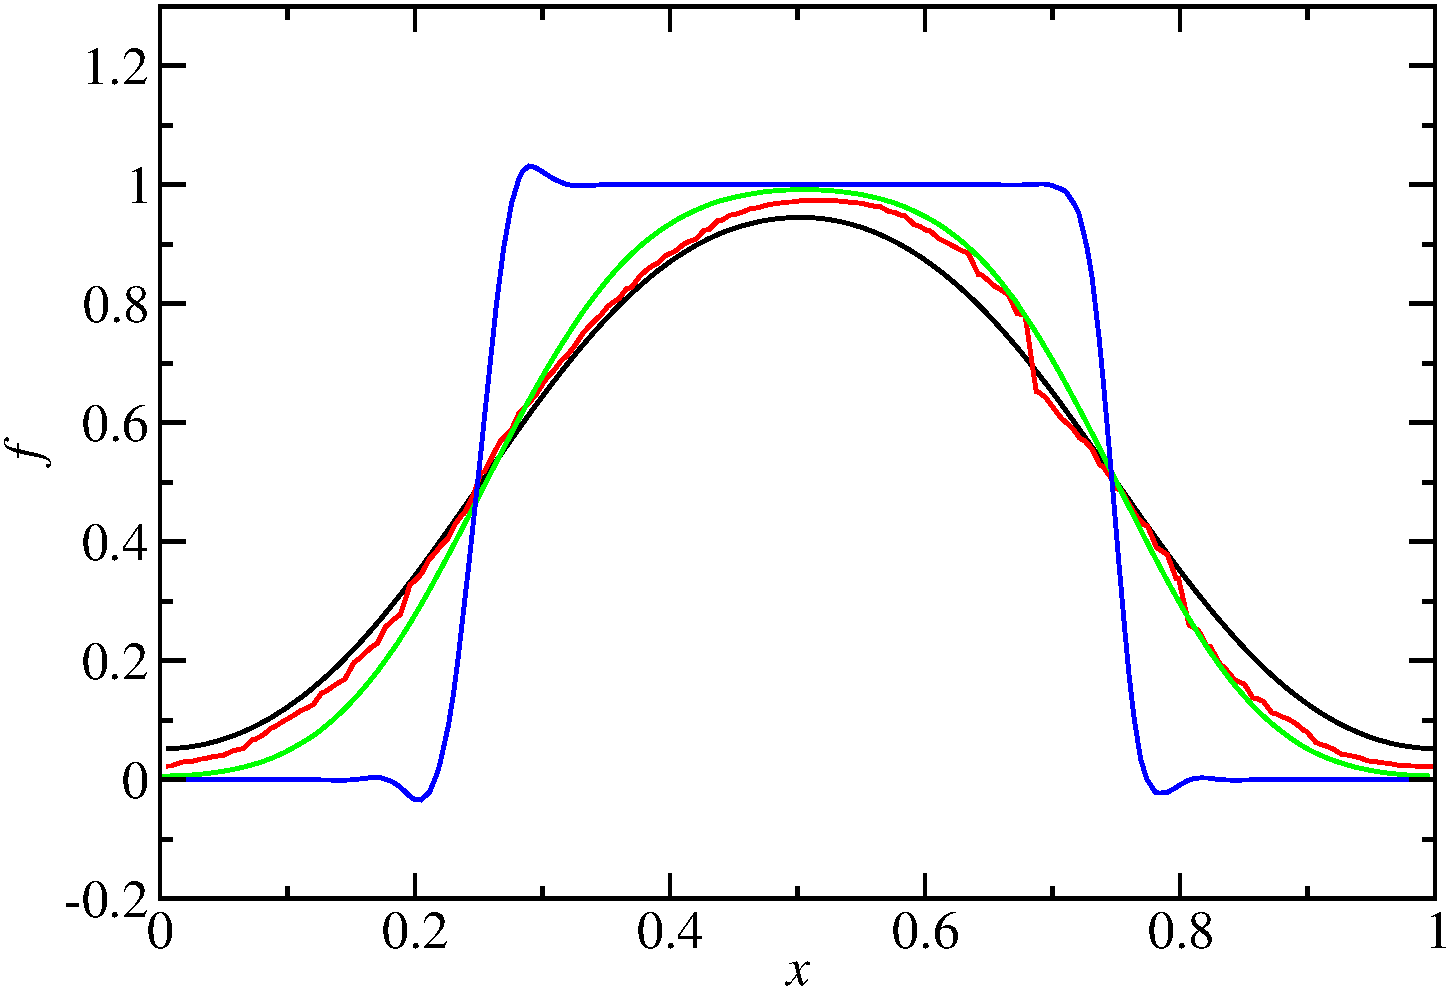
\includegraphics[width=\textwidth]{1D_final_pert}
  \end{minipage}
  \caption{Results for the advected step function. Field after one
    traversal of the cell. Left: regular particle distribution, right:
    distorted. Black: $\delta$ projection, red: FLIP, green:
    mass-$\delta$, blue: full mass. \label{fig:1D_final}}
\end{figure}


\begin{table}
  \centering
  \begin{minipage}{0.45\textwidth}
  \begin{tabular}{cccc}
    method & $E_1$ & $E_2$ & $L_2$
    \\
    \hline
    \hline
    $\delta$ &  $0$ &  $-29\%$ & $35\%$
    \\
    FLIP     &  $0$ &  $-25\%$ & $35\%$
           \\
    mass-$\delta$     &  $0$ &  $-21\%$ & $29\%$
    \\
    full mass     &  $0$ &  $0.85\%$ & $10\%$
    \\
    \hline
  \end{tabular}
  \end{minipage}
  \begin{minipage}{0.45\textwidth}
  \begin{tabular}{cccc}
    method & $E_1$ & $E_2$ & $L_2$
    \\
    \hline
    \hline
    $\delta$ &  $-0.24\%$ &  $-29\%$ & $35\%$
    \\
    FLIP     &  $0$ &  $-25\%$ & $35\%$
           \\
    mass-$\delta$     &  $0.7 \%$ &  $-20\%$ & $29\%$
    \\
    full mass     &  $-0.7\%$ &  $-4\%$ & $12\%$
    \\
    \hline
  \end{tabular}
  \end{minipage}
  \caption{Results for 1D spacing. Left table: regular, right: distorted\label{table:1D_final}}
\end{table}






\subsection{Zalesak's disk}
\label{sec:zalesak}

Let us consider a region with a color field $\alpha$ that has a value
of $1$ for points inside a domain and $0$ for points outside and which
is simply advected:
\begin{equation}
  \frac{d A}{d t} = 0 \qquad   \frac{d \bfr}{d t} = \bfu .
\end{equation}
%where the time derivative is the convective derivative:
%$d \alpha /dt = \partial \alpha / \partial t + (\mathbf{u} \cdot
%\nabla) \alpha$.

The domain is a circle with a slot. The circle's radius is given a
value of $R=0.5$, while the slot was a width of $1/6$, and a height of
$5/6$. The simulation box is a $(-1.5,1.5)\times(-1.5,1.5)$ square,
and the number of nodes is set to $90 \times 90$, so that the mesh
spacing is $H=3/90=1/30$, these are the same value as in
\cite{Idelsohn_2015}.  The time step is $\Delta t=0.01$, which
corresponds to $\mathrm{Co}_H := u (\Delta t) /H \approx 0.94$ for
nodes on the rim of the disk.

The velocity field is a pure rotation:
\begin{align}
  u_x &= -\omega y\\
  u_y &=  \omega x ,
\end{align}
where $\omega=2\pi/\tau$, and the period of rotation is set to
$\tau=1$.  Periodic boundary conditions are used in this simulation,
but this fact is not really important since the only region that is
actually moved is inside a circle of radius $1.4$, within a larger
simulation box, of size $3 \times 3$.

For the mesh, and also for the particles in the mass methods, we use
linear FE functions, as in the previous 1D example.  For all mass
methods, a moving Delaunay triangulation must be maintained for the
projection from the mesh to the particles. In addition to that, the
calculation of the corresponding mass matrix, and its inversion, is
needed for the full mass method.

Again, it would make little sense to project from and onto the mesh at
every time-step, but for benchmarking purposes.  As in the 1D case,
the FLIP idea of projecting only increments is not applied. Results
are given in Figure \ref{fig:zalesak}, showing contour plots for
values between $0.49$ and $0.51$ of the $\alpha$ field on the mesh
nodes.  We include the initial contour, the contour after one
revolution, $T=\tau$, and after two revolutions, $T=2\tau$.

On the top left contours are shown for the $\delta$ procedure, and at
the top right, for the FLIP procedure. Both are seen to greatly smear
out the initial slab. At the bottom left, the full-$\delta$ procedure
is show. This time, some remains of the slab are seen after one
revolution. Finally, the full mass projection (at the bottom right)
produces quite good profiles even after two revolutions.


% On the lower row show results are shown for a ``fine'' simulation,
% with $6$ particles per mesh node, or $h=H/\sqrt{6}$.  Results for a
% linear method (bottom left) are quite poor, but with quadratic mesh
% shape functions the simulation turns out to be quite satisfactory
% (bottom middle). This fact confirms the findings of
% Ref. \cite{Idelsohn_2015}, in which a large number of particles per
% node is used.  Finally, if the particle shape functions also satisfy
% quadratic consistency the contours (bottom right) are much
% improved. However, the computational costs are quite high for the
% latter, a fact that will be further explored later on.

% These results confirm our previous analysis on how the consistency of
% the spatial approximation should have a direct impact on the overall
% error of the simulation. From now on, the focus will therefore be on
% two particular implementations of projFEM: \emph{projFEMq},
% corresponding to the top right of Fig. \ref{fig:zalesak}, with
% quadratic shape functions both for the mesh and the particles, and as
% many particles as mesh nodes --- and
% %
% \emph{projFEM6}, corresponding to bottom middle of
% Fig. \ref{fig:zalesak}, with quadratic mesh shape functions, linear
% particle shape functions, and $6$ times more particles than mesh
% nodes.


\begin{figure}
  \centering
  \begin{minipage}{0.45\textwidth}
      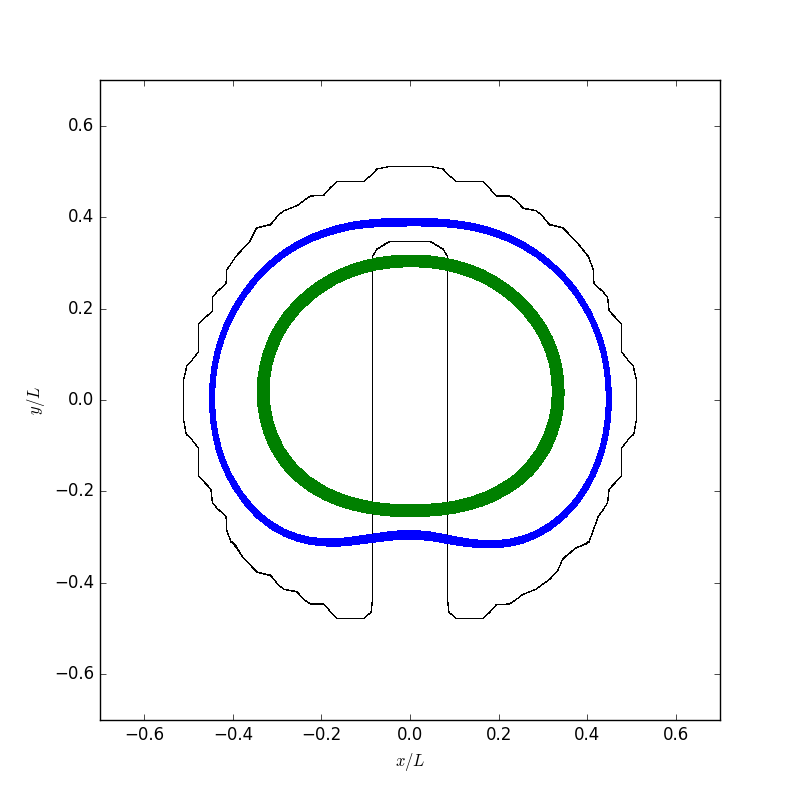
\includegraphics[width=\textwidth]{contours_delta}
  \end{minipage}
  \quad
  \begin{minipage}{0.45\textwidth}
      \includegraphics[width=\textwidth]{contours_flip}
  \end{minipage} \\
  \begin{minipage}{0.45\textwidth}
      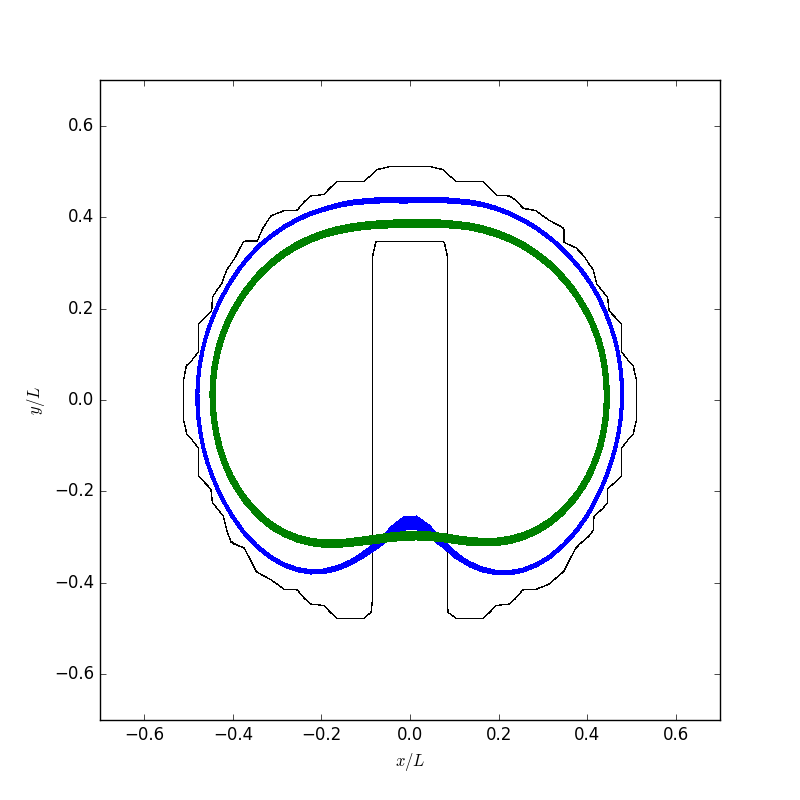
\includegraphics[width=\textwidth]{contours_full}
  \end{minipage}
  \quad
  \begin{minipage}{0.45\textwidth}
      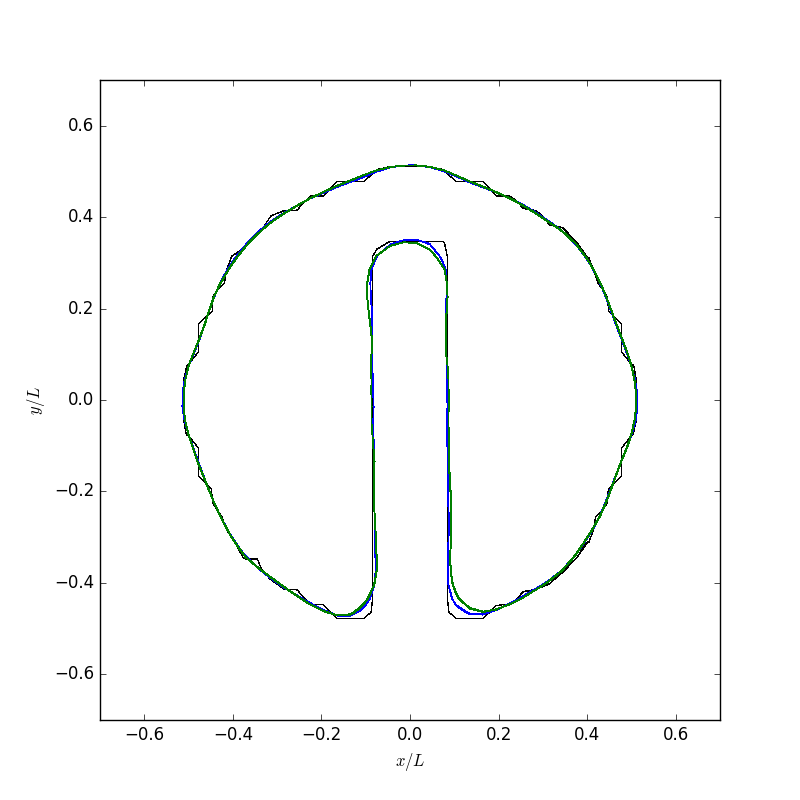
\includegraphics[width=\textwidth]{contours_full_full}
  \end{minipage}
  \caption{Results for the rotation of Zalesak's disk.  Isocontours for
  $\alpha \in ( 0.49 , 0.51 )$. Initial field in black, after one
  rotation in blue, after two in green. Top left: $\delta$ method. Top
  right: FLIP. Bottom left: mass-$\delta$. Bottom right: full mass.
  \label{fig:zalesak}}
\end{figure}

As in 1D, the good results of the full mass method maintaining the
plateaus are accompanied by undershoots below $0$ and overshoots above
$1$. In Figure \ref{fig:zalesak2} we show more detailed contours for
the full mass procedure.  The isocontour for $\alpha=0.5$ is shown
again, but the $\alpha=0$ contour reveals a corona of slightly
negative values, as low as $-0.05$ approximately.  Values of $\alpha$
about $1.05$ are also seen in the inner regions.

\begin{figure}
  \centering
  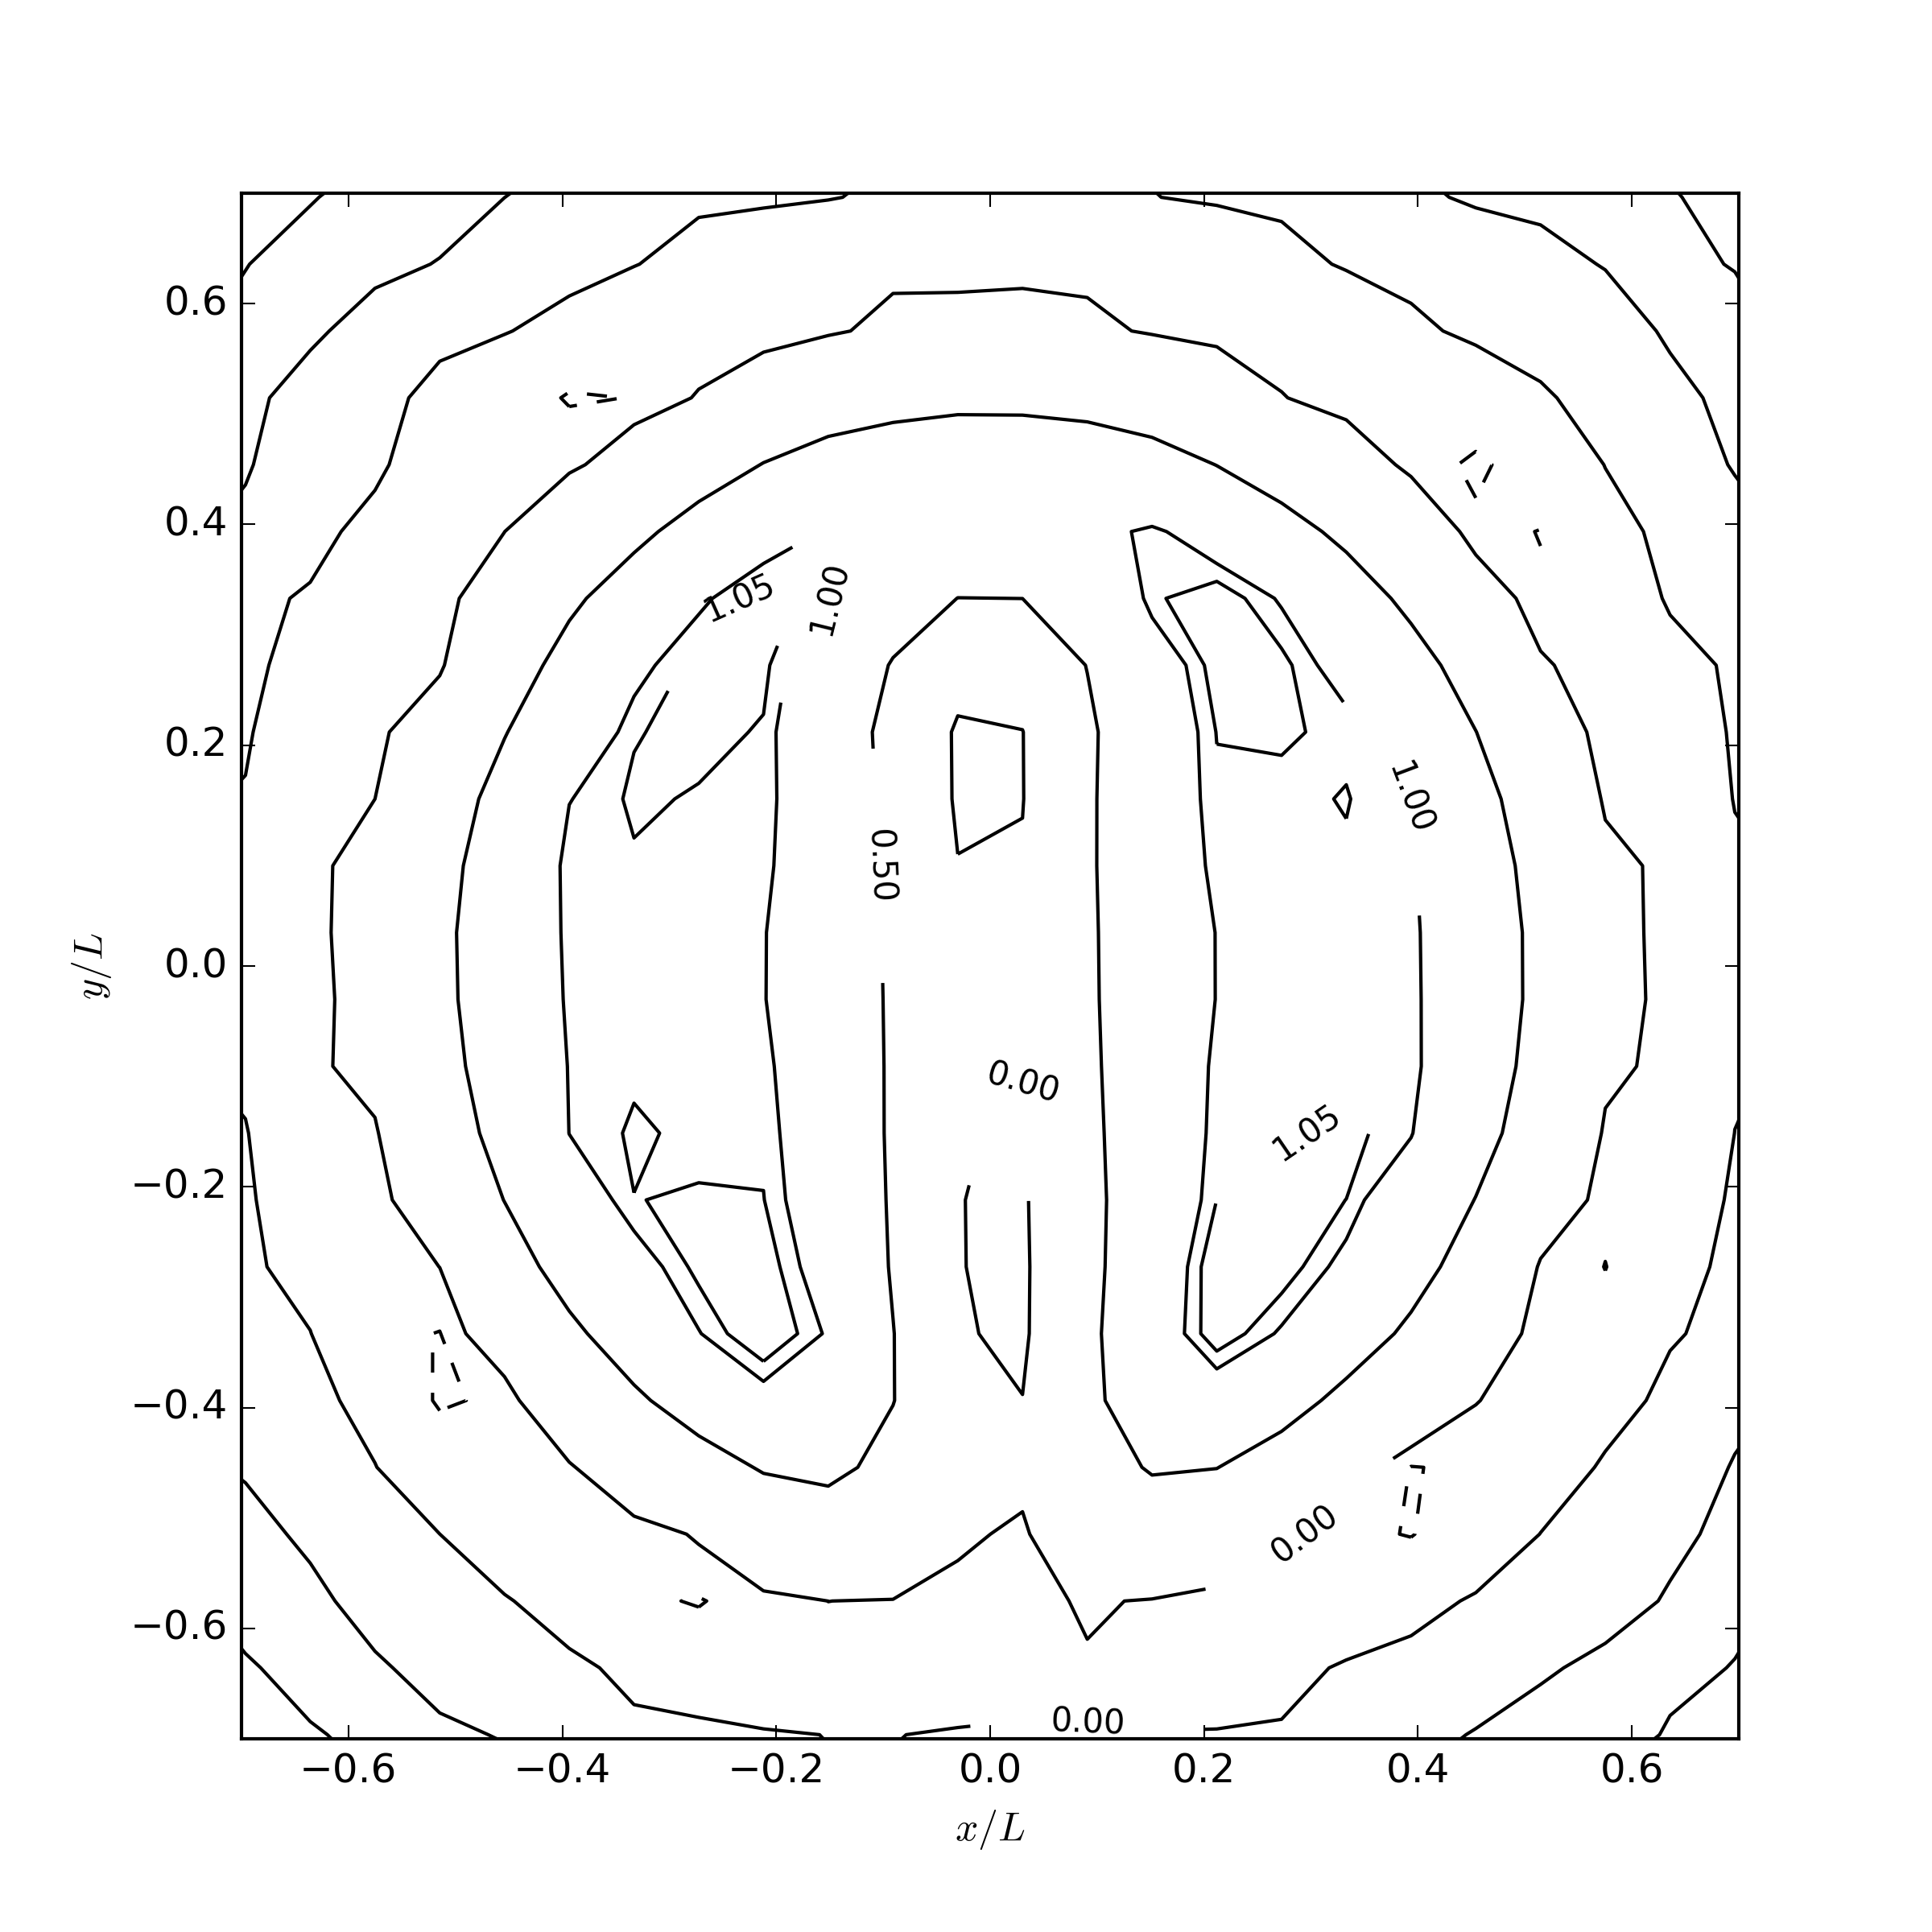
\includegraphics[width=0.5\textwidth]{final_contours_ffull}
  \caption{Results for the rotation of Zalesak's disk using the full
    mass method.  Isocontours for
    $\alpha \in ( -0.05, 0 , 0.5 , 1 , 1.05 )$ after two
    rotations. \label{fig:zalesak2}}
\end{figure}


We again employ the same error measures for our profiles. For the
relative $L_2$ distance we introduce a refinement, by comparing the
final profile and the one for a simulation in which the particle field
is simply advected. This way we subtract out the errors due to time
integration, by which particles' trajectories are not exactly
circles. These errors are quite small anyway.

\begin{table}
  \centering
  \begin{tabular}{cccc}
    method & $E_1$ & $E_2$ & $L_2$
    \\
    \hline
    \hline
    $\delta$ &  $-0.5\%$ &  $-29\%$ & $67\%$
    \\
    FLIP     &  $0.14\%$ &  $-61\%$ & $67\%$
    \\
    mass-$\delta$     &  $-0.5$ &  $-50\%$ & $61\%$
    \\
    full mass     &  $0.5\%$ &  $-9\%$ & $30\%$
    \\
    \hline
  \end{tabular}
  \caption{Results for the rotation of Zalesak's disk.\label{table:Zalesak}}
\end{table}




\subsection{Taylor-Green vortices}
\label{sec:TG}

The Taylor-Green vortex sheet is an analytic solution to the
Navier-Stokes equations for an incompressible Newtonian fluid:
\begin{equation}
  \frac{d \mathbf{u}}{d t} =  - \nabla p +  \nu \nabla^2 \mathbf{u}.
\end{equation}
%

The solution, with a periodic length of $L$, is the
velocity field
\begin{align}
\label{eq:TG_vel}
  \mathbf{u}_x &=  f(t) \sin (k x) \cos (k y) \\
  \mathbf{u}_y &= -f(t) \cos (k x) \sin (k y) ,\\
\end{align}
where $k=2\pi/L$, and the time-dependent prefactor function is given by
\[
f(t)=u_0 \exp\left( - 8 \pi^2 t^* /\mathrm{Re} \right) .
\]
The Reynolds number is defined as Re$:=u_0 L / \nu$, and the
dimensionless time is $t^* := t u_0/L$. We set $ u_0=1$, $L=1$, and
$\nu=0.005$, thus setting a Reynolds number of Re=$200$.

For the numerical solution of the Navier-Stokes equation, a standard
splitting approach is used, see \cite{codina_2001}.  The procedure is
a simple mid-point time integration, as in \cite{duque_2017b}. All
space derivatives are calculated on the mesh. As explained there, and
in \cite{Idelsohn_2015}, even this integrator, with $\Delta t^2$
accuracy, will result in a $\Delta t$ overall accuracy. This is
because the projection procedure causes a $\Delta t$ bottleneck in the
calculation. A possible remedy, proposed by \cite{duque_2017a}, is to
include higher order basis functions.  This idea is completely
compatible with the different assigments discussed, but for the sake
of simplicity we will not apply it here.

The main difference with the method in \cite{duque_2017b} is that the
FLIP incremential scheme (projecting only increments in fields at each
time step) is now applied to all simulation, both in FLIP assignment
(of course), and the others.

% In Fig. \ref{fig:TG} we show a snapshot of a simulation that has
% started from a regular arrangement, for a number of particles $N=20
% \times 20$, a time-step of $\Delta t^*=0.0125$ (corresponding to a
% Courant number of Co$_H=0.5$), at a reduced time $T^*=1$. The top left
% figure shows the particles' position and pressure field for the
% partFEM simulation.  At its right, the pressure field for the mesh in
% a projFEMq simulation is plotted.  The corresponding particles are
% plotted at the bottom left, with the same color code (actually, the
% pressure field is calculated only on the mesh, but here it has been
% interpolated on the particles for visualization purposes).  Finally,
% the figure on its right shows the particles for an projFEM6 simulation
% (the mesh result is visually very similar to the one above and is
% therefore not shown).

% \begin{figure}
%   \centering
%   \begin{minipage}{0.42\textwidth}
%     \includegraphics[width=\textwidth]{snap_fem1}
%   \end{minipage}
%   \quad
%   \begin{minipage}{0.42\textwidth}
%     \includegraphics[width=\textwidth]{snap_mesh_quad1}
%   \end{minipage}
%   \\
%   \begin{minipage}{0.42\textwidth}
%     \includegraphics[width=\textwidth]{snap_quad1}
%   \end{minipage}
%   \quad
%   \begin{minipage}{0.42\textwidth}
%     \includegraphics[width=\textwidth]{snap_femP1}
%   \end{minipage}
%   \caption{Results for the pressure field at $T^*=1$. From top left:
%     partFEM, projFEMq (field on the mesh), projFEMq (field on the
%     particles), projFEM6 (field on the particles).\label{fig:TG}}
% \end{figure}


In order to quantify the accuracy of the different methods, 
%in \del{Figure} \new{Fig.} \ref{fig:TG-L2} 
the relative $L_2$ distance between the velocity field obtained by
simulation and its exact value is computed:
\begin{equation}
\label{eq:L2_error}
L_2:=
\sqrt{%
  \frac{
    \sum_{i=1}^N 
    V_i
    \left|
      \bfu(\bfr_i) - \bfu_i
    \right|^2
  }{
    \sum_{i=1}^N 
    V_i
    |\bfu(\bfr_i)|^2
  }
} ,
\end{equation}
where $\bfu(\bfr_i)$ is the exact velocity field as in
(\ref{eq:TG_vel}), evaluated on particle $i$ position. The same
measure may be evaluated for mesh nodes, with very similar
results.

This error is expected to start at a very low value and increase
approximately linearly as the simulation proceeds. In order to compare
between methods, in Fig. \ref{fig:L2_x} the value of this error at
$T^*=1$ is plotted.  At this time, $f(T)=\exp(-8\pi^2 / 200 )=0.67 $,
so that the velocity field should have decreased to about $67\%$ of
its initial value.

The error for the velocity field (left subfigure) is seen to decrease
with $\Delta t$. The interparticle and mesh spacing is decreased as
$\Delta t$ does, in order to fix a Courant number of Co$_H=0.5$ (the
number of nodes and particles therefore increases quadratically with
$1/\Delta t$).
Like in Zalesak's disk test, there are as many particles as nodes. The
particles are created at the beginning of the simulation and moved
according to the velocity field. As expected, the order of convergence
of the error roughly agrees with a $\Delta t^1$ power in all cases.
Results from the full mass procedure are much more accurate. However,
at finer resolutions the latter results cross over to a power law with an
exponent lower than $1$, for reasons that are not clear.


%  This is very likely due to the integrator for the
% pressure not being a mid-point one, as the one for the velocity, and
% should be improved with a more sophisticated algorithm.

\begin{figure}
  \centering 
  \includegraphics[width=0.7\textwidth]{L2_x}
  \caption{%
    $L_2$ error of the velocity  field at
    time $T^*=1$, versus time step $\Delta t$.  Black circles: $\delta$
    method, red squares: FLIP, green diamonds: mass-$\delta$, blue triangles:
    full mass. The triangle shows a $\Delta t^1$ power-law.
    \label{fig:L2_x}
  }
\end{figure}

Despite its superior performance, the full mass is clearly more
costly computationally than the alternatives. It therefore seems
interesting to plot the error as a function of CPU time.
A bad scaling as the number of nodes and particles is increased
would make this procedure less appealing. However,
Fig. \ref{fig:L2_x_vs_T} makes clear that the full mass
procedure scales similarly to other procedures, with $L_2$ roughly
proportional to $\Delta t^{1/4}$, while being about ten times
more accurate for the same computational cost. Similarly
to the previous Figure, the full mass results cross over to a power
law with an exponent lower than $1/4$.

The CPU run times clearly depend on the machine used, but a faster one
would likely accelerate all simulations by a similar factor. This
would result in a horizontal translation of all the curves in a
logarithmic scale. Results do depend on the particular linear algebra
algorithm used, details can be found in Appendix \ref{sec:numerical}.

One may therefore conclude from these observations that the higher
computational cost of a full mass method will be compensated by its
higher accuracy.

\begin{figure}
  \centering
  \includegraphics[width=0.7\textwidth]{L2_x_vs_T}
  \caption{%
    $L_2$ error of the velocity  field at
    time $T^*=1$, versus CPU time in seconds  Black circles: $\delta$
    method, red squares: FLIP, green diamonds: mass-$\delta$, blue triangles:
    full mass. The triangle shows a $\Delta t^1$
    power-law.
    \label{fig:L2_x_vs_T}  }
\end{figure}



\section{Conclusions}
\label{sec:conclusions}


We have described several assignment, or projection, procedures by
which field information may be transferred between particles and mesh.
We have focused on four procedures: the simplest $\delta$ method, the
FLIP method, the mass-$\delta$ method and the full mass method.

Each method is tested against several requirements: conservativity,
which makes sure that the total integral of a field is not changed;
stability, that ensures that the integral of the square of a field
decreases upon projection; and preservation of information, which
means that the assignment procedure carried twice leaves the field
values invariant if the particles and the mesh have the same
positions.

We have tested the method in 1D and 2D advection problems.
Conservativity is satisfied exactly by construction in the FLIP method,
and rather well satisfied in the other cases.  Stability is satisfied
in all four methods, but the full mass method is seen to be superior
in producing a smaller decrease. On the other hand, it also leads to
higher over- and undershoots at sharp interfaces.

Finally, the full mass method is clearly superior in our CFD
simulations of the Taylor-Green vortex sheet, where an approximate
ten-fold increase in accuracy is achieved for the same simulation
clock time.  The puzzling moderation of the convergence rates at
higher resolutions is under study. Results (not shown here) with the
quadratic basis functions described in \cite{duque_2017a} are free
from this effect, and show power law convergences at higher exponents:
$L_2 \sim \Delta t^2$, and $L_2 \sim \mathrm{CPU}^{-1/2}$.


The final conclusion is that the full mass method should be seriously
considered as an assignment procedure, despite its inherent higher
computational complexity.


\section*{Acknowledgments}

We wish to thank Prof. David Le Touz\'e for his suggestions regarding
the FLIP method. We also thank Prof. Michael Schick for hosting a
research stay, during which this work was finished. The research
leading to these results has received funding from the Ministerio de
Econom\'{\i}a y Competitividad of Spain (MINECO) under grants
TRA2013-41096-P ``Optimizaci\'on del transporte de gas licuado en
buques LNG mediante estudios sobre interacci\'on fluido-estructura''
and FIS2013-47350-C5-3-R ``Modelizaci\'on de la Materia Blanda en
M\'ultiples escalas''.



%\bibliographystyle{authordate1}
\bibliography{PiC,sme_pdes,comp_geom}



\appendix



\section{Numerical methods}
\label{sec:numerical}

For all computational geometry procedures the CGAL 4.7 libraries
(\cite{CGAL}) are used.  In particular, the 2D Periodic Delaunay
Triangulation package, overloading the vertex base to contain the
relevant fields, and the face base to contain information relevant to
the edges.

The Eigen 3.0 linear algebra libraries (\cite{Eigen}) are also
employed.  For the small linear algebra problem involved in the
calculation of the $A$ coefficients, SVD is used, with automatic rank
detection. For the large problems involved in the Galerkin procedure,
the sparse matrix package is used. The linear systems are solved
iteratively for pFEM, by the BiCGSTAB method.  For projFEM a direct
method is employed, with best results obtained using the CHOLMOD
(\cite{cholmod}) routines of the suitesparse project (through Eigen
wrappers for convenience, class CholmodSupernodalLLT). Slightly worse
results are obtained with eigen's build-in SimplicialLDLT class.

Our computations took place on a 4-core Pentium 4 machine with 16 Gb
RAM. The code employed, named polyFEM, may be found in
(\cite{polyFEM}) under an open source license.



\section{Quadrature}
\label{sec:quadrature}

As explained in the main text, the ``mass'' assignments involve
integrals as in Equation (\ref{eq:proj}).

In this work, the $A(\bfr)$ is a piece-wise linear function, that
connects the values of at the particles $A_\mu$. The fact that the
locations of mesh nodes and particles do not match makes the integral
somewhat cumbersome to evaluate.  We have therefore implemented a
simple quadrature rule. It is best visualized in 1D, see Figure
\ref{fig:quadrature}. For the interval between node $i$ and $i+1$
function $A(x)$ is evaluated at $x_i$, $x_{i+1}$ and the position in
between. The resulting three values are then fit to a parabola, whose
overlap integral (functional scalar product) with $\phi_i$ is trivial
to evaluate. As shown in the Figure, if no particles lie on the
interval, this approximation is exact: the parabola will degenerate
to a line in this case. If some particle lies in the interval the
result will be, in general, an approximation.  For each node $i$ there
will be an additional integration from $i-1$ to $i$.

The same procedure is carried out in 2D, as also depicted in Figure
\ref{fig:quadrature}. The view is from above, and for simplicity only
2D points are drawn, not functions. Function $A(\bfr)$ is evaluated at
the nodes of the triangle that connects node $i$ and two of its
neighbors in the triangulation. In addition, it is also evaluated at
the mid-points of each segment. With these six values, a recontructing
quadratic function is found, whose overlap integral with $\phi_i$ is
trivial. Similar to the 1D case, if the mesh triangle is fully
contained within a particle triangle, the integral is exact (since in
this case $A$ is linear). If, however, the mesh triangle is crossed by
at least one edge of the particle triangulation, the result will be
approximate.  For each node $i$ the integration must be performed over
all its other incident triangles.  An equivalent procedure is applied
in the inverse procedure of (\ref{eq:proj2}).


\begin{figure}
  \centering
  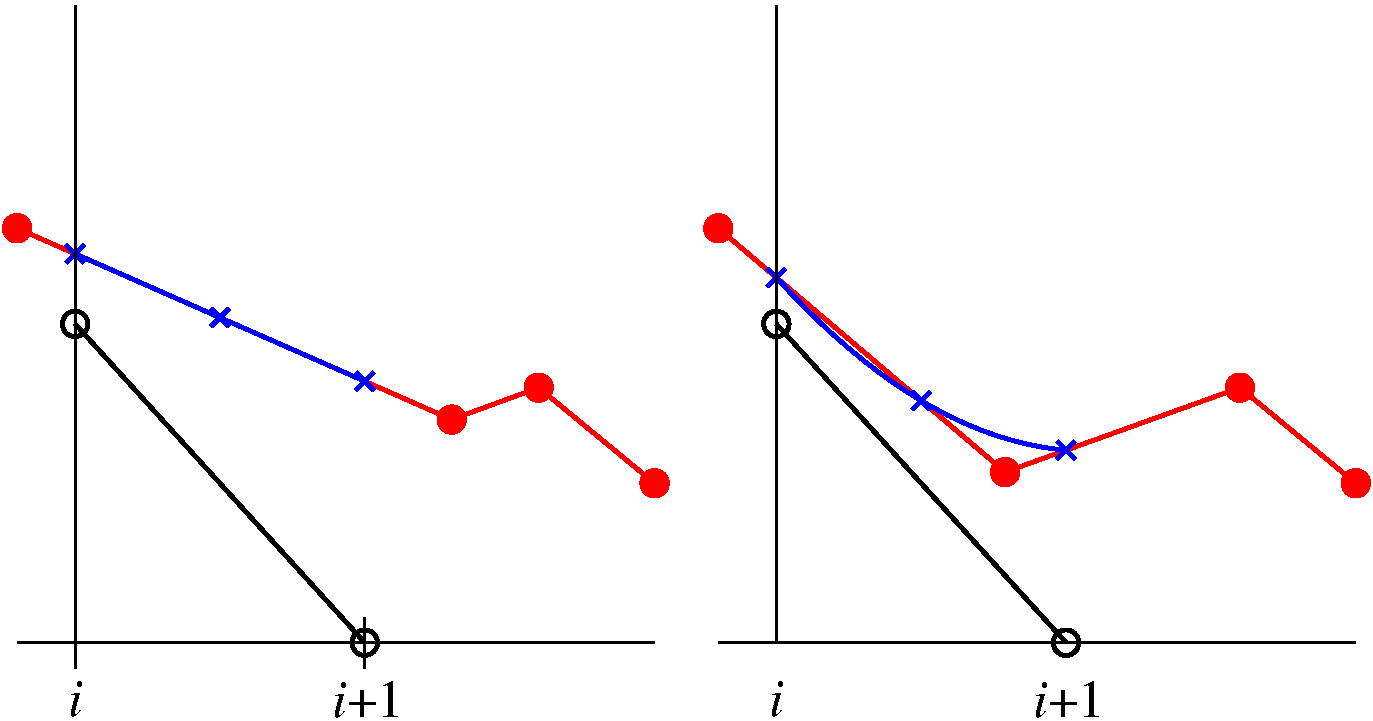
\includegraphics[width=0.45\textwidth]{quadrature} $\qquad$
  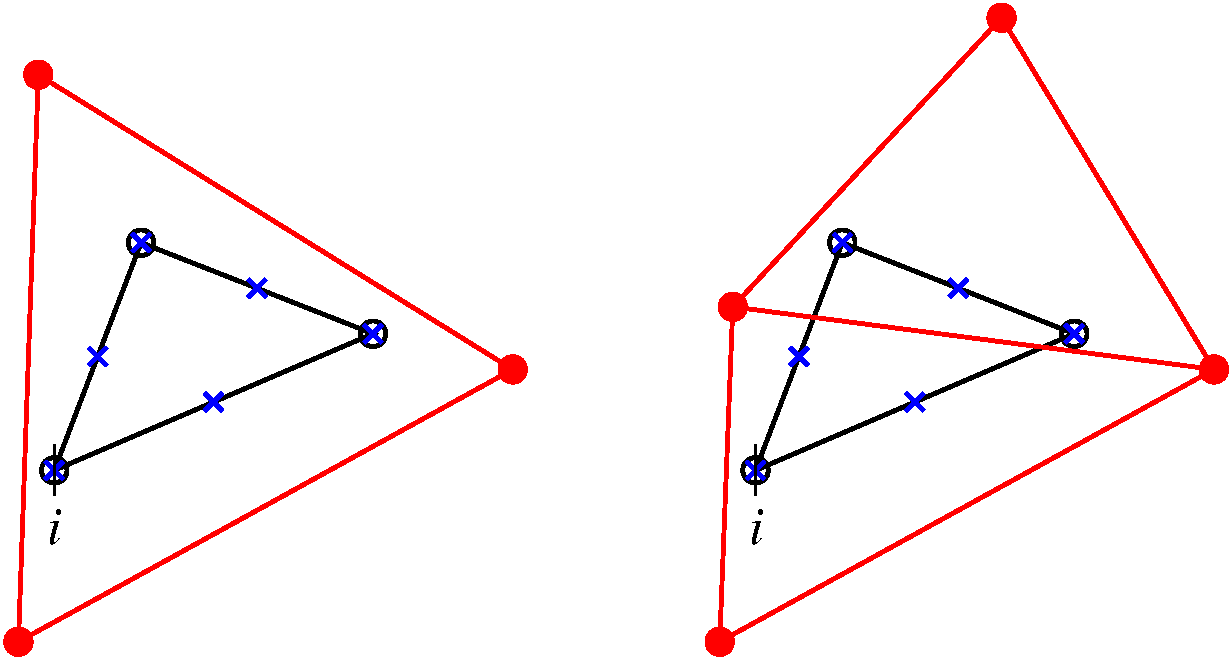
\includegraphics[width=0.45\textwidth]{quadrature_2D}
  \caption{%
    Illustration of the quadrature used in 1D (left two figures), and
    2D (right two figures).
    In 1D, $\phi_i(x)$ is shown as a black line, and $A(x)$
    as a red line. The quadratic approximation to the latter is shown
    as a blue line. In 2D, the black empty circles show the position of nodes, red
    full circles, the position of particles. Blue crosses are quadrature
    points in both cases.
    \label{fig:quadrature}}
\end{figure}



\end{document}
